\documentclass[letterpaper,onecolumn,titlepage]{Ythesis}
\usepackage[utf8]{inputenc}
\usepackage{tikz}
\usepackage{array,multirow}
\usepackage{subcaption}
\usepackage{subfiles}
\usepackage{url}
\usepackage{amsmath}
\usepackage{float}
\usepackage{graphicx}
\graphicspath{{figures}{.figures}}
\usepackage[backend=bibtex, style=numeric-comp]{biblatex}
\bibliography{glasslab_viz}



\title{Make any stupid plot you want}
\author{Hannah Aizenman}
\committee{Dr. Michael Grossberg (Advisor), Dr. Robert Haralick, Dr. Lev Manovich, Dr. Huy Vo}
\submitted{}
\abstract{}
\begin{document}
\makefrontmatter

\section{Introduction}
\label{sec:introduction}
\begin{figure}
    \includegraphics[width=.5\textwidth]{figures/intro/dubois_bookplate}
    \caption{This collection of visualizations is the inside cover art of W. E. B. Du Bois's Data Portraits\cite{duboiscenterattheuniversityofmassachusettsBoisDataPortraits2018}}
\end{figure}



\cite{huntermatplotlib2007}
\cite{duboiscenterattheuniversityofmassachusettsBoisDataPortraits2018}

\begin{verbatim}
make any stupid plot you want in robust & rigourous way
        * need rich description langauge + right choice of paradigm (functional) 
        * ability to mathemetaically formalize/conceptual framework for doing this
        * data -> artist, need to preserved the structure of the data moreso than the data 
            * how points are connected to each other
    * targeted implementation rather than protocal (numpy)
        * visualization libraries bound to the datastructures (concrete implementation)
            * encode a lot of assumptions about data in the data structure
            * MPL assume x/y plotted in order you want them in 
            * topology makes the assumptions explicit
            * explicit->math->functional  
    * spell out the layers of visualization libaries:
        * Data + computation -> visualization composites -> drawing library
        * domain specific library
        * utility library <- formalize this piece (SciPy Diagram)
    * viz - Munzner + Bertin
    * functional programming makes sense 
\end{verbatim}


\begin{figure}
    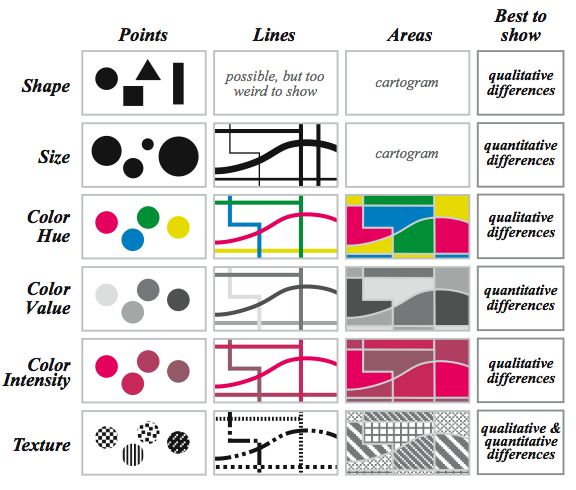
\includegraphics{figures/intro/retinal_variables}
    \label{fig:retinal_variable}
    \caption{\cite{krygierMakingMapsVisual2005}}
\end{figure}
\cite{bertinSemiologyGraphicsDiagrams2011}


\begin{figure}
    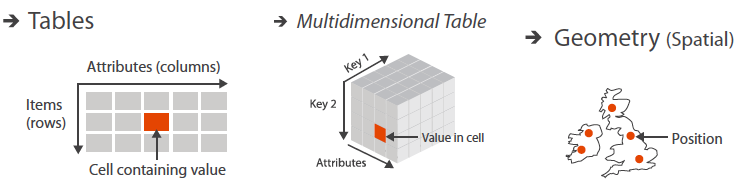
\includegraphics{figures/intro/munzner_datatypes}
    \label{fig:munzner_datatypes}
    \caption{Keys are unique lookup values used to find individual observations in the dataset. Keys are positional references, and can be coordinates on a map or unique values such as a primary key in a database or a (time, latitude, longitude) index in a data cube. Image modified from a diagram from Munzner's website\cite{munznerChDataAbstraction}}
\end{figure}
\cite{munznerWhatDataAbstraction2014}

\printbibliography
\end{document}